\documentclass[11pt]{article}
\usepackage{geometry}                
\geometry{letterpaper}                   

\usepackage{graphicx}
\usepackage{amssymb}
\usepackage{epstopdf}
\usepackage{natbib}
\usepackage{amssymb, amsmath}
\usepackage{wrapfig}





%\title{Title}
%\author{Name 1, Name 2}
%\date{date} 

\begin{document}



\thispagestyle{empty}

\begin{center}

\includegraphics[width=5cm]{ETHlogo.eps}

\bigskip


\bigskip


\bigskip


\LARGE{ 	Lecture with Computer Exercises:\\ }
\LARGE{ Modelling and Simulating Social Systems with MATLAB\\}

\bigskip

\bigskip

\small{Project Report}\\

\bigskip

\bigskip

\bigskip

\bigskip


\begin{tabular}{|c|}
\hline
\\
\textbf{\LARGE{Cholera Epidemic in Haiti 2010}}\\
\\
\hline
\end{tabular}
\bigskip

\bigskip

\bigskip

\LARGE{Nicolas Stocker 

Benedict Borer

Benjamin Pluess 

Lukas Buehler}



\bigskip

\bigskip

\bigskip

\bigskip

\bigskip

\bigskip

\bigskip

\bigskip

Zurich\\
\today\\
\end{center}



\newpage

%%%%%%%%%%%%%%%%%%%%%%%%%%%%%%%%%%%%%%%%%%%%%%%%%

\newpage
\section*{Agreement for free-download}
\bigskip


\bigskip


\large We hereby agree to make our source code for this project freely available for download from the web pages of the SOMS chair. Furthermore, we assure that all source code is written by ourselves and is not violating any copyright restrictions.

\begin{center}

\bigskip


\bigskip


\begin{tabular}{@{}p{3.3cm}@{}p{6cm}@{}@{}p{6cm}@{}}
\begin{minipage}{3cm}

\end{minipage}
&
\begin{minipage}{6cm}
\vspace{2mm} \large Nicolas Stocker 


 \vspace{\baselineskip}

\end{minipage}
&
\begin{minipage}{6cm}

\large Benjamin Pluess

\end{minipage}
\end{tabular}

\bigskip
\bigskip
\bigskip

\begin{tabular}{@{}p{3.3cm}@{}p{6cm}@{}@{}p{6cm}@{}}
\begin{minipage}{3cm}

\end{minipage}
&
\begin{minipage}{6cm}
\vspace{2mm} \large Benedict Borer 


 \vspace{\baselineskip}

\end{minipage}
&
\begin{minipage}{6cm}

\large Lukas Buehler

\end{minipage}
\end{tabular}


\end{center}
\newpage

%%%%%%%%%%%%%%%%%%%%%%%%%%%%%%%%%%%%%%%



% IMPORTANT
% you MUST include the ETH declaration of originality here; it is available for download on the course website or at http://www.ethz.ch/faculty/exams/plagiarism/index_EN; it can be printed as pdf and should be filled out in handwriting


%%%%%%%%%% Table of content %%%%%%%%%%%%%%%%%

\tableofcontents

\newpage

%%%%%%%%%%%%%%%%%%%%%%%%%%%%%%%%%%%%%%%



\section{Abstract}

\section{Individual contributions}

\section{Introduction and Motivations}
\textit{The Shock}

\begin{wrapfigure}{r}{5cm}
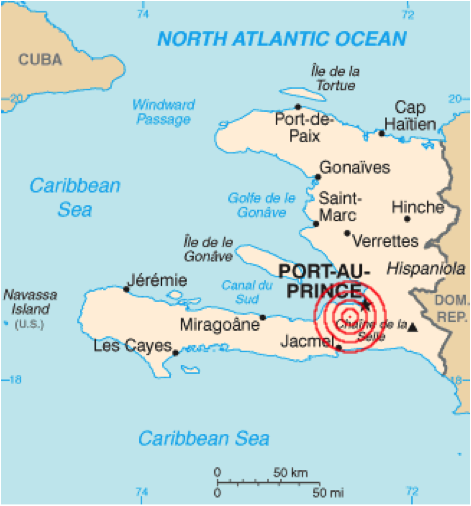
\includegraphics[scale=0.8]{Bilder/KarteHaiti.png}
\caption{Hier steht die Beschreibung des Bildes}%
\end{wrapfigure}
12. January 2010, 16.53 local time in Haiti: during one minute the earth is shaking with magnitude 7.0  (on the Moment magnitude scale) with an epicentre 25 Km west of Haiti’s capital Port-au-Prince. Followed by at least 52 aftershocks  this earthquake is the most dramatic in the 21. Century: the Haitian government estimated that 316’000 people had died , one million people lost their home  and 3.2 million are directly affected.
\\[1em]
\noindent \textit{Geological overview}

The quake was located on the active plate boundary with the Caribbean Tectonic Plate shifts eastwards relative to the North American Plate. This causes a highly dangerous strike-slip-fault system here with the southern active Enriquillo-Plantain-Garden-fault. The quake is caused by a rupture of this system, which has been blocked for the last 2500 years, loading stress
\\[1em]
\noindent\textit{Primary impacts}

As Haiti is one of the poorest country in the Western Hemisphere  the economy is highly vulnerable to natural disasters. In addition to earthquakes, the “island of Hispaniola” shared by the Dominican Republic and Haiti, has often been stroked by Hurricanes. 
\newline
The huge devastation and damage in the whole country, but especially in the region of the capital, destroy not only human life, furthermore infrastructure, which would have been necessary to respond to the disaster. Not only all hospitals in the capital, as well air, water and land transport facilities and the communication system was destroyed. As well a lot off the public and government buildings were damaged (e.g. the National Assembly, the Palace of Justice and the Supreme Court)
\\[1em]
\noindent\textit{The time afterwards}

In the following months after the earthquake many people slept in the streets because their houses has been destroyed or they were feared that their buildings won’t survive upcoming aftershocks. Slow distribution of recourses resulted in violence and some people began with plundering.
\newline
The earthquake destroyed thousands of families and made collapse a whole social system and destroyed economic interactions in a country. Anarchy and a right-free area was the result. Haitians dramatic fight for survival began in the silent seconds after the earthquake and still goes on.
\\[1em]
\noindent\textit{Upcoming problem: Cholera}

During the period of reconstruction in October 2010 Haiti was confronted by a new dangerous problem: a cholera epidemic broke out! 
\newline
Cholera is a bacterial infection caused by a bacterium named as “Vibro cholerae”. The symptoms are mainly watery diarrhoea and vomiting. The transmission occurs generally by drinking infected water. Cholera doesn’t have to be lethal but requires an appropriate treatment in a hospital. In Haiti in January 2012 some 7025 deaths by Cholera have been reported 
The source of the illness still is not clearly identified, but localized in de Artibonite River about 100 Km north of Port-Au-Prince (The affected victims had drunk water from the infected river). Some UN investigators did researches, hoping to find the real source from the Epidemic and they are guessing the initial strain was imported by UN peacekeeper from Nepal . The Nepali soldiers may be the source of the outbreak as wastewater from their outhouses at their base flowed into and contaminated the Artibonite River  . However who brought the origin strain to Haiti is not of primary importance, rather than to control the plague and this is still one of the most important priority nowadays in Haiti.
\\[1em]
\noindent\textit{Motivation}

By the end of October 2010 the Cholera epidemic accomplished four out of ten Haitian’s departments: Artibonite, Centre, Nord and Ouest. That includes as well the Capital , especially the slum district “Cité Soleil” . In the following days Cholera was spread all over the country and infected thousands of peoples. The tragedy of Haiti is not only a “simple” earthquake; it is more a battle rebuilding a country affected by complicating circumstances such as the Cholera Epidemic. 
\newline
Our aim is to understand the fast spreading of the dangerous illness Cholera and to implement a mathematical model, which is able to predict the expansion of such an epidemic in space and time. We believe to help getting a deeper understanding of the interaction of a human – environment interaction and so to do our part for protecting human lives in further catastrophic events.


\section{Description of the Model}

\section{Implementation}

\section{Simulation Results and Discussion}

\section{Summary and Outlook}



\noindent\textit{Outlook}

In response to the cholera outbreak, the Haiti government and partner agencies initiated emergency public health response activities aimed at treating suspected cholera cases and preventing new ones. Response activities included mass media cholera campaigns through radio and hygiene promotion activities by community health workers, distribution of water purification tablets and soap, and limited distribution of oral rehydration solution (ORS) sachets. (Quelle: http://www.ncbi.nlm.nih.gov/pmc/articles/PMC3310585/?tool=pubmed)

Regarding to the mass media campaign, it seems helpful to know how  the cholera bacteria would distribute in waterways. With our model it is possible to make a forecast about the distribution in water ways. Based on that knowledge the protection of population is directly improved and should be used when cholera is threatening human beings.


\section{References}






\end{document}  
